% Created by tikzDevice version 0.7.0 on 2015-01-08 13:31:53
% !TEX encoding = UTF-8 Unicode
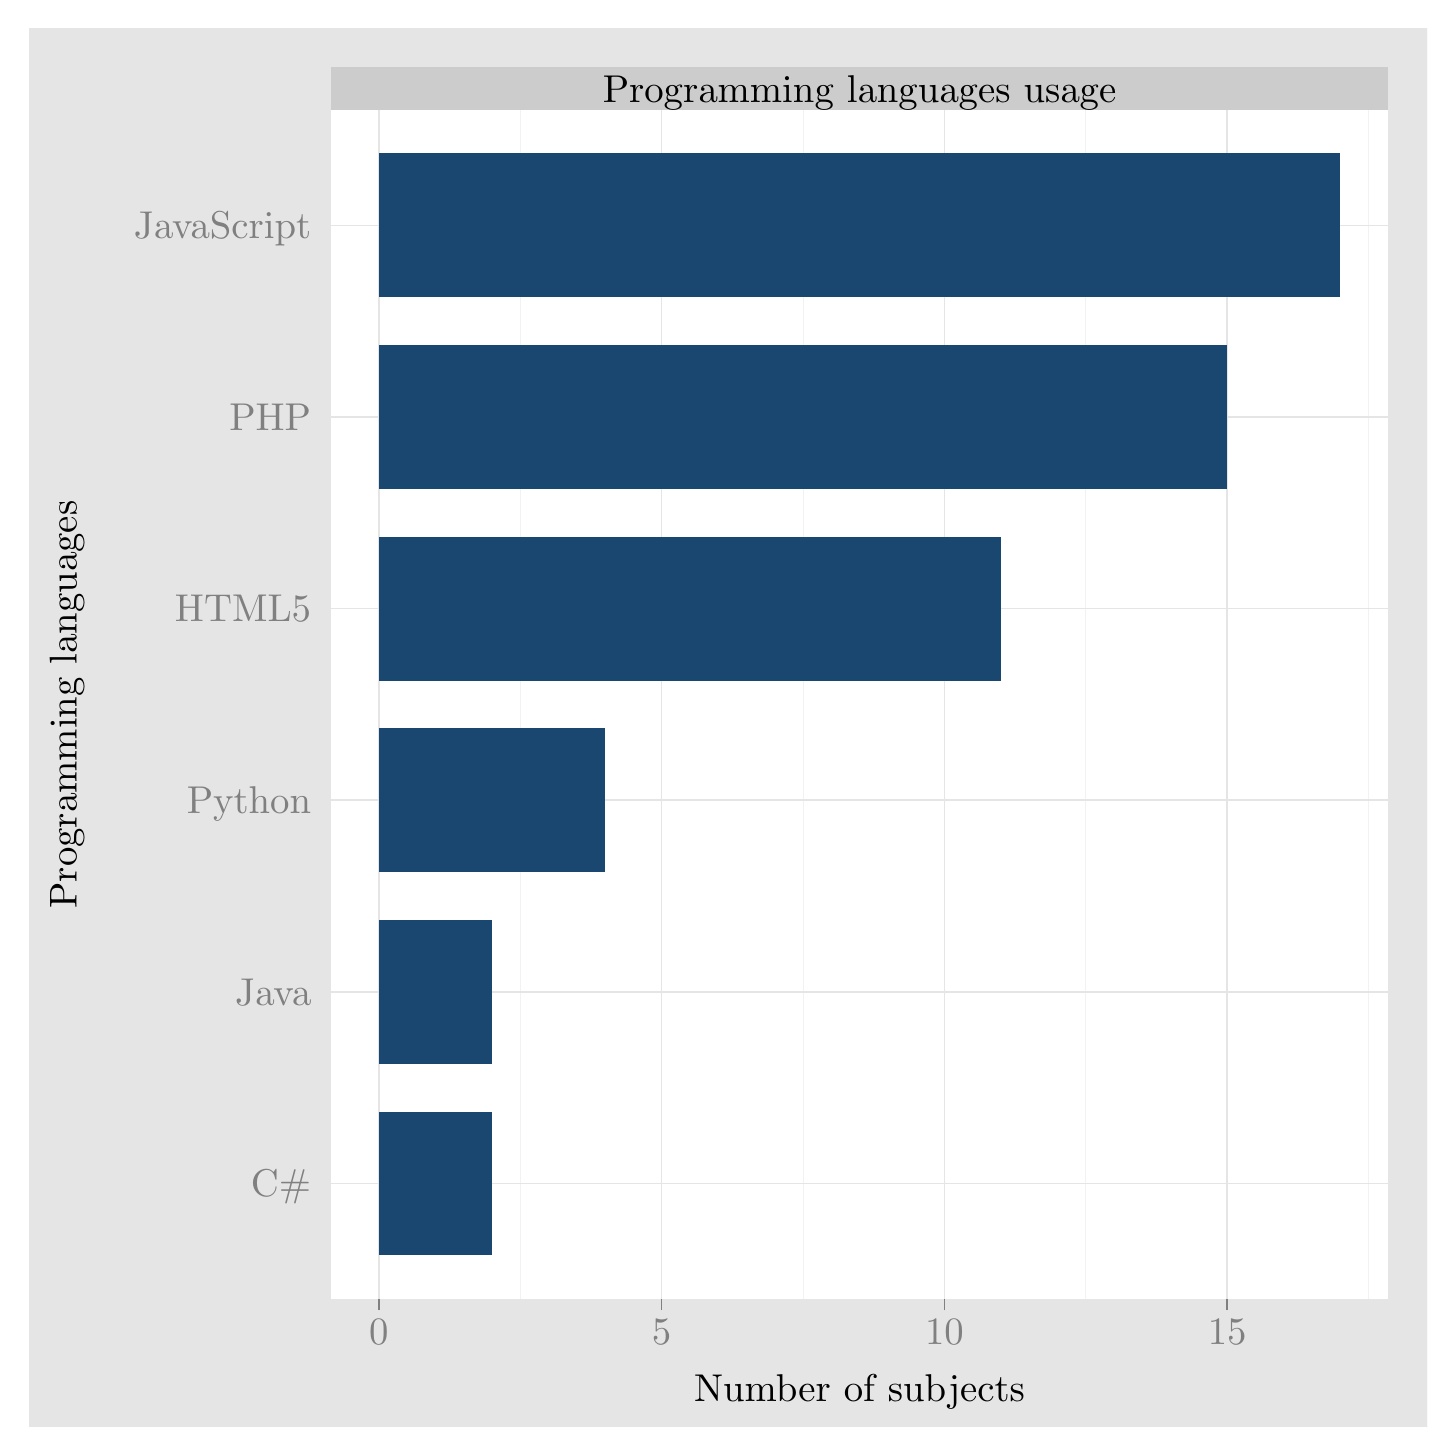
\begin{tikzpicture}[x=1pt,y=1pt]
\definecolor[named]{fillColor}{rgb}{1.00,1.00,1.00}
\path[use as bounding box,fill=fillColor,fill opacity=0.00] (0,0) rectangle (505.89,505.89);
\begin{scope}
\path[clip] (  0.00,  0.00) rectangle (505.89,505.89);
\definecolor[named]{drawColor}{rgb}{1.00,1.00,1.00}
\definecolor[named]{fillColor}{rgb}{0.90,0.90,0.90}

\path[draw=drawColor,line width= 0.6pt,line join=round,line cap=round,fill=fillColor] (  0.00, -0.00) rectangle (505.89,505.89);
\end{scope}
\begin{scope}
\path[clip] (109.54, 46.65) rectangle (491.66,476.00);
\definecolor[named]{fillColor}{rgb}{1.00,1.00,1.00}

\path[fill=fillColor] (109.54, 46.65) rectangle (491.66,476.00);
\definecolor[named]{drawColor}{rgb}{0.95,0.95,0.95}

\path[draw=drawColor,line width= 0.3pt,line join=round] (177.99, 46.65) --
	(177.99,476.00);

\path[draw=drawColor,line width= 0.3pt,line join=round] (280.16, 46.65) --
	(280.16,476.00);

\path[draw=drawColor,line width= 0.3pt,line join=round] (382.34, 46.65) --
	(382.34,476.00);

\path[draw=drawColor,line width= 0.3pt,line join=round] (484.51, 46.65) --
	(484.51,476.00);
\definecolor[named]{drawColor}{rgb}{0.90,0.90,0.90}

\path[draw=drawColor,line width= 0.6pt,line join=round] (109.54, 88.20) --
	(491.66, 88.20);

\path[draw=drawColor,line width= 0.6pt,line join=round] (109.54,157.45) --
	(491.66,157.45);

\path[draw=drawColor,line width= 0.6pt,line join=round] (109.54,226.70) --
	(491.66,226.70);

\path[draw=drawColor,line width= 0.6pt,line join=round] (109.54,295.95) --
	(491.66,295.95);

\path[draw=drawColor,line width= 0.6pt,line join=round] (109.54,365.20) --
	(491.66,365.20);

\path[draw=drawColor,line width= 0.6pt,line join=round] (109.54,434.45) --
	(491.66,434.45);

\path[draw=drawColor,line width= 0.6pt,line join=round] (126.90, 46.65) --
	(126.90,476.00);

\path[draw=drawColor,line width= 0.6pt,line join=round] (229.08, 46.65) --
	(229.08,476.00);

\path[draw=drawColor,line width= 0.6pt,line join=round] (331.25, 46.65) --
	(331.25,476.00);

\path[draw=drawColor,line width= 0.6pt,line join=round] (433.42, 46.65) --
	(433.42,476.00);
\definecolor[named]{fillColor}{rgb}{0.10,0.28,0.44}

\path[fill=fillColor] (126.90, 62.23) rectangle (167.77,114.17);

\path[fill=fillColor] (126.90,131.48) rectangle (167.77,183.42);

\path[fill=fillColor] (126.90,200.73) rectangle (208.64,252.67);

\path[fill=fillColor] (126.90,269.98) rectangle (351.69,321.92);

\path[fill=fillColor] (126.90,339.23) rectangle (433.42,391.17);

\path[fill=fillColor] (126.90,408.48) rectangle (474.29,460.42);
\end{scope}
\begin{scope}
\path[clip] (  0.00,  0.00) rectangle (505.89,505.89);
\definecolor[named]{fillColor}{rgb}{0.80,0.80,0.80}

\path[fill=fillColor] (109.54,476.00) rectangle (491.66,491.66);
\definecolor[named]{drawColor}{rgb}{0.00,0.00,0.00}

\node[text=drawColor,anchor=base,inner sep=0pt, outer sep=0pt, scale=  1.40] at (300.60,479.01) {Programming languages usage};
\end{scope}
\begin{scope}
\path[clip] (  0.00,  0.00) rectangle (505.89,505.89);
\definecolor[named]{drawColor}{rgb}{0.50,0.50,0.50}

\node[text=drawColor,anchor=base east,inner sep=0pt, outer sep=0pt, scale=  1.40] at (102.42, 83.38) {C\#};

\node[text=drawColor,anchor=base east,inner sep=0pt, outer sep=0pt, scale=  1.40] at (102.42,152.63) {Java};

\node[text=drawColor,anchor=base east,inner sep=0pt, outer sep=0pt, scale=  1.40] at (102.42,221.88) {Python};

\node[text=drawColor,anchor=base east,inner sep=0pt, outer sep=0pt, scale=  1.40] at (102.42,291.13) {HTML5};

\node[text=drawColor,anchor=base east,inner sep=0pt, outer sep=0pt, scale=  1.40] at (102.42,360.38) {PHP};

\node[text=drawColor,anchor=base east,inner sep=0pt, outer sep=0pt, scale=  1.40] at (102.42,429.63) {JavaScript};
\end{scope}
\begin{scope}
\path[clip] (  0.00,  0.00) rectangle (505.89,505.89);
\definecolor[named]{drawColor}{rgb}{0.50,0.50,0.50}

\path[draw=drawColor,line width= 0.6pt,line join=round] (126.90, 42.38) --
	(126.90, 46.65);

\path[draw=drawColor,line width= 0.6pt,line join=round] (229.08, 42.38) --
	(229.08, 46.65);

\path[draw=drawColor,line width= 0.6pt,line join=round] (331.25, 42.38) --
	(331.25, 46.65);

\path[draw=drawColor,line width= 0.6pt,line join=round] (433.42, 42.38) --
	(433.42, 46.65);
\end{scope}
\begin{scope}
\path[clip] (  0.00,  0.00) rectangle (505.89,505.89);
\definecolor[named]{drawColor}{rgb}{0.50,0.50,0.50}

\node[text=drawColor,anchor=base,inner sep=0pt, outer sep=0pt, scale=  1.40] at (126.90, 29.89) {0};

\node[text=drawColor,anchor=base,inner sep=0pt, outer sep=0pt, scale=  1.40] at (229.08, 29.89) {5};

\node[text=drawColor,anchor=base,inner sep=0pt, outer sep=0pt, scale=  1.40] at (331.25, 29.89) {10};

\node[text=drawColor,anchor=base,inner sep=0pt, outer sep=0pt, scale=  1.40] at (433.42, 29.89) {15};
\end{scope}
\begin{scope}
\path[clip] (  0.00,  0.00) rectangle (505.89,505.89);
\definecolor[named]{drawColor}{rgb}{0.00,0.00,0.00}

\node[text=drawColor,anchor=base,inner sep=0pt, outer sep=0pt, scale=  1.40] at (300.60,  9.41) {Number of subjects};
\end{scope}
\begin{scope}
\path[clip] (  0.00,  0.00) rectangle (505.89,505.89);
\definecolor[named]{drawColor}{rgb}{0.00,0.00,0.00}

\node[text=drawColor,rotate= 90.00,anchor=base,inner sep=0pt, outer sep=0pt, scale=  1.40] at ( 17.70,261.32) {Programming languages};
\end{scope}
\end{tikzpicture}
